\subsection{Gerarchia di tipi} % (fold)
\label{sub:gerarchia_di_tipi}
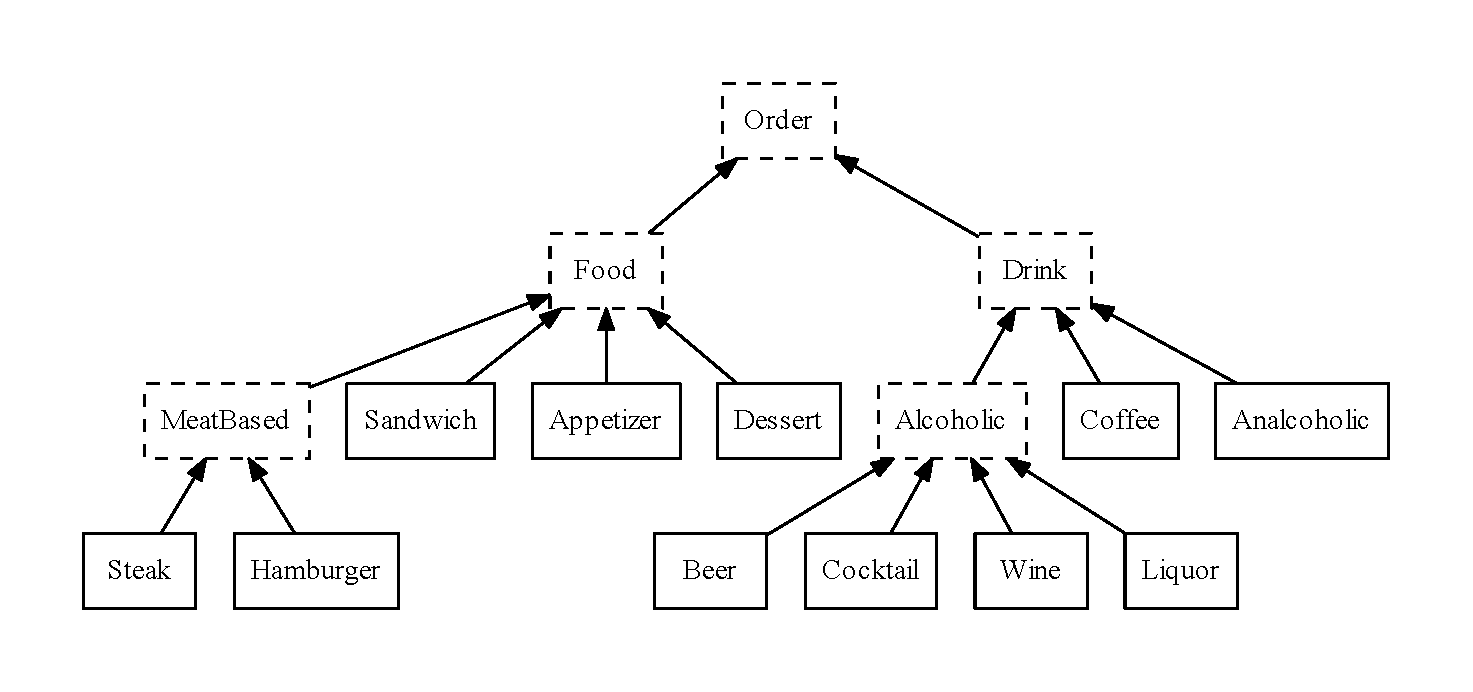
\includegraphics[width=\linewidth]{gerarchia.pdf}
\paragraph{Informazioni Generali} % (fold)
\label{par:informazioni_generali}
La gerarchia modella le ordinazioni inviate alla cucina del ristorante. Radicata nella classe polimorfa astratta \code{Order}, si dirama in due direzioni, \code{Food} e \code{Drink}, associate rispettivamente a ordinazioni di piatti e bevande. Il polimorfismo è dato da alcuni metodi virtuali, descritti in seguito, che forniscono funzionalità di copia e confronto polimorfi, e permettono di ricavare informazioni esplicite sul tipo degli oggetti. La gerarchia è fortemente estensibile sia "in orizzontale", aggiungendo nuovi sottotipi alle classi base presenti, sia "in verticale", fornendo sottotipi alle classi più derivate.
% paragraph informazioni_generali (end)
\paragraph{Membri Statici} % (fold)
\label{par:membri_statici}
La classe \code{Order} comprende anche dei membri statici, che forniscono due tipi di funzionalità:
\begin{itemize}
	\item Forniscono informazioni complessive sulla gerarchia.
	\item Forniscono informazioni e funzionalità relative ad un tipo a partire da una stringa.
\end{itemize}
In questo modo è possibile sfruttare una sorta di polimorfismo che non richiede un oggetto di invocazione.
% paragraph membri_statici (end)
\subsubsection{Order} % (fold)
\label{ssub:order}
\paragraph{Campi Dati} % (fold)
\label{par:campi_dati}
La classe \code{Order} incapsula informazioni di base relative ad un ordine attraverso tre campi dati privati di istanza:
\begin{itemize}
	\item \code{table}: \code{unsigned int}, il numero del tavolo,
	\item \code{item}: \code{std::string}, il nome della pietanza,
	\item \code{quantity}: \code{unsigned int}, il numero di porzioni
\end{itemize}
È presente un campo dati privato statico, \code{class_name}, che incapsula il nome della classe sottoforma di stringa. Sono inoltre presenti 4 metodi statici privati che permettono l'accesso a degli oggetti che, concettualmente, dovrebbero essere campi statici, ma per motivi progettuali (spiegati in seguito) sono allocati sullo heap e vengono acceduti attraverso puntatori di classe statica:
\begin{itemize}
	\item \code{static std::vector<std::string> &abstracts()}\newline
	Metodo che ritorna un \code{std::vector} contenente i nomi delle classi astratte derivate da \code{Order} sottoforma di stringa.
	\item \code{static std::vector<std::string> &types()}\newline
	Metodo che ritorna un \code{std::vector} contenente i nomi delle classi istanziabili derivate da \code{Order} sottoforma di stringa.
	\item \code{static std::multimap<std::string, std::pair<DetailType, std::string>> &info()}\newline
	Metodo che ritorna una \code{std::multimap} che associa a ciascun tipo derivato da \code{Order} la forma ed il nome dei dettagli specifici per quel tipo.
	\item \code{static std::map<std::string, std::function<DeepPtr<Order>(unsigned int,}\newline
	\code{const std::string &, unsigned int, const std::vector<std::string> &)>> &make()}\newline
	Metodo che ritorna una \code{std::map} che associa a ciascun tipo derivato da \code{Order} una funzione che agisce da costruttore, ritornando un puntatore smart ad un nuovo oggetto.
\end{itemize}
% paragraph campi_dati (end)
\paragraph{Metodi} % (fold)
\label{par:metodi}
Per l'interazione con gli oggetti sono disponibili $13$ metodi pubblici di istanza (virtuali e non) che comprendono un costruttore ed il distruttore, a cui vanno aggiunti il costruttore di copia e l'operatore di assegnazione di copia standard forniti dal compilatore. I metodi di istanza sono:
\begin{itemize}
	\item \code{Order(unsigned int, const std::string &, unsigned int)}\newline
	Costruisce un oggetto inizializzando i campi dati al valore del rispettivo parametro, in ordine.
	\item \code{virtual ~Order() = default}\newline
	Distruttore di default, dichiarato virtuale.
	\item \code{virtual Order *clone() const = 0}\newline
	Metodo di copia "standard", dichiarato virtuale puro per permettere la costruzione di copia polimorfa.
	\item \code{unsigned int getTable() const}\newline
	Getter per il campo dati \code{table}.
	\item \code{std::string getItem() const}\newline
	Getter per il campo dati \code{item}.
	\item \code{unsigned int getQuantity() const}\newline
	Getter per il campo dati \code{quantity}.
	\item \code{void setQuantity(unsigned int)}\newline
	Setter per il campo dati \code{quantity}.
	\item \code{virtual std::string getClassName() const}\newline
	Metodo virtuale che ritorna il nome della classe sottoforma di stringa.
	\item \code{virtual bool isA(const std::string &) const}\newline
	Metodo virtuale il cui parametro, \code{type}, è interpretato come il nome di una classe \code{Type}, e ritorna true se e solo se il tipo dinamico di \code{*this} è un sottotipo di \code{Type}.
	\item \code{virtual std::vector<std::string> getDetails() const = 0}\newline
	Metodo virtuale puro che ritorna un elenco di "dettagli" relativi all'ordine, cioè informazioni aggiuntive specifiche associate al tipo di pietanza ordinata.
	\item \code{virtual void setDetails(const std::vector<std::string> &) = 0}\newline
	Metodo virtuale puro speculare a \code{getDetails()}, permette di modificare le informazioni aggiuntive.
	\item \code{virtual bool operator==(const Order &) const}\newline
	Operatore di uguaglianza, dichiarato virtuale per tenere in considerazione dei ettagli relativi alle sottoclassi. L'implementazione "parziale" fornita da \code{Order} confronta i rispettivi tipi e i campi dati.
	\item \code{bool operator!=(const Order &) const}\newline
	Operatore di disuguaglianza, dichiarato non virtuale in quanto si basa sull'operatore di uguaglianza. Ritorna \code{true} se e solo se l'operatore di uguaglianza ritorna \code{false}.
\end{itemize}
Sono inoltre presenti 4 metodi pubblici statici che agiscono da getter per i "campi dati statici" allocati sullo heap:
\begin{itemize}
	\item \code{static const std::vector<std::string> &getAbstracts();}\newline
	Getter per \code{abstracts()}.
	\item \code{static const std::vector<std::string> &getTypes();}\newline
	Getter per \code{types()}.
	\item \code{static const std::multimap<std::string, std::pair<DetailType, std::string>> &getInfo();}\newline
	Getter per \code{info()}.
	\item \code{static const std::map<std::string, std::function<DeepPtr<Order>(unsigned int,}\newline
	\code{const std::string &, unsigned int, const std::vector<std::string> &)>> &getMake();}\newline
	Getter per \code{make()}.
\end{itemize}
% paragraph metodi (end)
\paragraph{Classi Annidate} % (fold)
\label{par:classi_annidate}
È presente una classe annidata protetta, \code{Empty}, la quale non ha campi dati, ed ha due costruttori:
\begin{itemize}
 	\item \code{Empty(const std::string &);}\newline
 	Il parametro viene interpretato come il nome di una classe astratta derivata da \code{Order}, e viene aggiunto a \code{abstracts()}.
	\item \code{Empty(const std::string &, const std::vector<std::pair<DetailType, std::string>> &,}\newline
	\code{const std::function<DeepPtr<Order>(unsigned int, const std::string &, unsigned int,}\newline
	\code{const std::vector<std::string> &)> &);}\newline
	Il primo parametro, \code{type}, viene interpretato come il nome di un tipo derivato da \code{Order}, e viene aggiunto a \code{types()}; il secondo, \code{details}, come un elenco di coppie (forma, nome) associate a dettagli di una classe derivata, e quindi ogni suo elemento viene agiunto a \code{info()} utilizzando \code{type} come chiave; infine, il terzo parametro, \code{constructor}, viene interpretato come una funzione che agisce da costruttore, e quindi viene aggiunto a \code{make()} utilizzando ancora \code{type} come chiave.
\end{itemize}
È inoltre presente una scoped enumeration, \code{DetailType}, che rappresenta le varie forme che possono assumere i dettagli aggiunti dalle classi derivate:
\begin{itemize}
	\item \code{DetailType::Choice}, una scelta fra due alternative.
	\item \code{DetailType::SmallText}, un breve testo (ad esempio una dimensione, o una temperatura).
	\item \code{DetailType::LargeText}, un testo più lungo (ad esempio una descrizione o un elenco).
\end{itemize}
% paragraph classi_annidate (end)
\paragraph{"Polimorfismo su Stringhe"} % (fold)
\label{par:_polimorfismo_su_stringhe_}
Per assicurare il corretto popolamento di \code{abstracts()}, \code{types()}, \code{info()}, e \code{make()} è necessario che ciascuna classe derivata (anche indirettamente) da \code{Order} abbia un campo dati statico, possibilimente privato, di tipo \code{Empty}, e che esso sia inizializzato con il costruttore adeguato: per le classi astratte quello ad un parametro, a cui va passato il nome della classe, mentre per le classi istanziabili quello a tre parametri, a cui vanno passati il nome della classe, l'elenco dei dettagli, come coppie (forma, nome), e una funzione che agisca da costruttore. In particolare, i dettagli nell'elenco devono essere nello stesso ordine in cui vengono ritornati dal metodo \code{getDetails()}. Questo sistema garantisce che i 4 container siano popolati correttamente all'avvio dell'applicazione grazie al fatto che i campi dati statici sono costruiti prima dell'esecuzione della funzione \code{main()}, ed essendo completamente automatico esonera l'utente della gerarchia dall'invocazione di un'ipotetica funzione \code{setup()}. Il tutto si basa sulla garanzia che i 4 container siano costruiti prima di essere popolati, ed è per questo che vengono costruiti sullo heap ed acceduti attraverso puntatori di classe statica locali ai metodi di accesso: essendo di classe statica, le inizializzazioni dei puntatori vengono eseguite solo una volta, la prima volta che le funzioni vengono invocate, cioè la prima volta che un campo statico di tipo \code{Empty} viene costruito. D'altro canto, essendo allocati sullo heap andrebbero deallocati con \code{delete}, cosa che non avviene, ma siccome andrebbero deallocati dopo l'esecuzione della \code{main} questo non consiste in un memory leak, perchè in questo momento la memoria viene comunque reclamata dal sistema operativo. 
% paragraph _polimorfismo_su_stringhe_ (end)
\paragraph{RTTI su stringhe} % (fold)
\label{par:rtti_su_stringhe}
I metodi \code{getClassName()} e \code{isA()} forniscono una versione basata su stringhe dei meccanismi di RTTI. Considerando una reference valida \code{o} di tipo \code{Order &} (oppure, per un ragionamento analogo, un puntatore valido di tipo \code{Order *}), l'invocazione \code{o.getClassName()} ritorna una stringa analoga a quella ritornata da \code{typeid(o).name()}, con la particolarità che la prima è fissata dal programmatore, mentre la seconda è implementation defined. In modo simile, se \code{type} è una stringa contenente il nome di una classe \code{Type}, l'invocazione \code{o.isA(type)} è analoga a \code{dynamic_cast<Type *>(&o)!=nullptr}, ma in questo caso la differenza, più marcata, è che \code{isA()} "agisce" su stringhe, mentre il \code{dynamic_cast} "agisce" su tipi.
% paragraph rtti_su_stringhe (end)
% subsubsection order (end)
\subsubsection{Food} % (fold)
\label{ssub:food}
La classe astratta \code{Food}, derivata da \code{Order}, rappresenta ordini di piatti. Presenta un campo dati aggiuntivo \code{without}, dotato di getter e setter, che rappresenta parti del piatto che il cliente ha chiesto di escludere; per tenere in considerazione il nuovo campo dati è presente un costruttore adeguato. Il metodo \code{clone()}, pur rimanendo virtuale puro, subisce overriding per modificare il tipo di ritorno (che è quindi covariante). Gli altri metodi virtuali sono reimplementati come da aspettative.
% subsubsection food (end)
\subsubsection{MeatBased} % (fold)
\label{ssub:meatbased}
La classe astratta \code{MeatBased}, derivata da \code{Food}, rappresenta ordini di piatti il cui ingrediente principale è un tipo di carne, e per questo ha un ulteriore campo dati \code{temperature}, dotato di getter e setter, che rappresenta la temperatura di cottura della carne; è quindi fornito un costruttore adeguato. Il metodo \code{clone()} subisce ancora override, ma non viene ancora implementato. Gli altri metodi virtuali sono reimplementati come da aspettative.
% subsubsection meatbased (end)
\subsubsection{Steak, Hamburger} % (fold)
\label{ssub:steak_hamburger}
Le classi \code{Steak} e \code{Hamburger}, derivate da \code{MeatBased}, rappresentano ordini di piatti il cui ingrediente principale è rispettivamente una bistecca o un hamburger. Non presentano campi dati aggiuntivi, ma \code{Steak} non fa uso del campo dati \code{without} di \code{Food}; di conseguenza, \code{Hamburger} utilizza il costruttore di \code{MeatBased}, mentre \code{Steak} ne fornisce uno ad hoc. Per lo stesso motivo, solo \code{Steak} reimplementa \code{getDetails()} e \code{setDetails()}. Gli altri metodi virtuali sono reimplementati come da aspettative.
% subsubsection steak_hamburger (end)
\subsubsection{Sandwich} % (fold)
\label{ssub:sandwich}
La classe \code{Sandwich}, derivata da \code{Food}, rappresenta ordini di piatti basati su sandwich. Non presenta campi dati aggiuntivi, e di conseguenza utilizza il costruttore di \code{Food}. Per lo stesso motivo, non reimplementa \code{getDetails()} e \code{setDetails()}. Gli altri metodi virtuali sono reimplementati come da aspettative.
% subsubsection sandwich (end)
\subsubsection{Appetizer, Dessert} % (fold)
\label{ssub:appetizer_e_dessert}
Le classi \code{Appetizer} e \code{Dessert}, derivate da \code{Food}, rappresentano ordini di antipasti e dolci, rispettivamente. Ciascuna ha un campo dati aggiuntivo, \code{sauces} e \code{with} nell'ordine, con getter e setter, ed entrambe non fanno uso del campo dati \code{without} di \code{Food}. Per questo forniscono entrambe costruttori, ed entrambe reimplementano \code{getDetails()} e \code{setDetails()}. Gli altri metodi virtuali sono reimplementati come da aspettative.
% subsubsection appetizer_e_dessert (end)
\subsubsection{Drink} % (fold)
\label{ssub:drink}
La classe astratta \code{Drink}, derivata da \code{Order}, rappresenta ordini di bevande; non presenta nessun campo dati aggiuntivo, e quindi utilizza il costruttore ereditato da \code{Order}. Il metodo \code{clone()}, subisce overriding per modificare il tipo di ritorno ma non viene implementato, come non vengono implementati \code{getDetails()} e \code{setDetails()}. Gli altri metodi virtuali sono reimplementati come da aspettative.
% subsubsection drink (end)
\subsubsection{Alcoholic} % (fold)
\label{ssub:alcoholic}
La classe astratta \code{Alcoholic}, derivata da \code{Drink}, rappresenta ordini di bevande alcoliche; non presenta nessun campo dati aggiuntivo, e quindi utilizza il costruttore ereditato da \code{Drink}. Il metodo \code{clone()}, subisce overriding per modificare il tipo di ritorno ma non viene implementato, come non vengono implementati \code{getDetails()} e \code{setDetails()}. Gli altri metodi virtuali sono reimplementati come da aspettative.
% subsubsection alcoholic (end)
\subsubsection{Beer, Cocktail, Wine, Liquor} % (fold)
\label{ssub:beer_cocktail_wine_liquor}
Le classi \code{Beer}, \code{Cocktail}, \code{Wine}, e \code{Liquor}, derivate da \code{Alcoholic}, rappresentano ordini di birre, cocktail, vini, e liquori, rispettivamente. Ciascuna ha un campo dati aggiuntivo, \code{size}, \code{garnish}, \code{vintage} e \code{ice} nell'ordine, con getter e setter, e per questo forniscono tutte costruttori. I metodi virtuali sono reimplementati come da aspettative.
% subsubsection beer_cocktail_wine_liquor (end)
\subsubsection{Coffee, Analcoholic} % (fold)
\label{ssub:coffe_analcoholic}
Le classi \code{Coffee} e \code{Analcoholic}, derivate da \code{Drink}, rappresentano ordini di caffè e bibite analcoliche, rispettivamente. Ciascuna ha un campo dati aggiuntivo, \code{notes} e \code{ice} nell'ordine, con getter e setter, e per questo forniscono tutte costruttori. I metodi virtuali sono reimplementati come da aspettative.
% subsubsection coffe_analcoholic (end)
% subsection gerarchia_di_tipi (end)